Se realizaron ejecuciones del algoritmo para distintos datasets de grafos de diversos tamaños y tipo de construcción, y se tomaron los tiempos de las mismas utilizando el $\delta1$ y $\delta2$ como funci'on objetivo y comparando ambos resultados.
La siguiente tabla muestra los tamaños de clique hallado con la Heurística Constructiva y tamaño del clique máximo para ambos $\delta$.
\footnote{
En http://cs.hbg.psu.edu/benchmarks/clique.html	

SAN (From Laura Sanchis laura@cs.colgate.edu) Instances based on her "Test Case Construction for Vertex Cover Problem," DIMACS Workshop on Computational Support for Discrete Mathematics, March 1992 along with more recent work that will be part of a technical report to be published. The generator generates instances with known clique size.

BROCK (From Mark Brockington brock@cs.ualberta.ca) Instances from Mark Brockington and Joe Culberson's generator that attempts to $"hide"$ cliques in a graph where the expected clique size is much smaller. For more instances, see their generator in graph/contributed/brockington.

PHAT (From Patrick Soriano and Michel Gendreau patrick@crt.umontreal.ca) Random problems generated with the p hat generator which is a generalization of the classical uniform random graph generator. Uses 3 parameters: n, the number of nodes, and a and b, two density parameters verifying 0 $<=$ a $<=$ b $<=$ 1. Generates problem instances having wider node degree spread and larger clique sizes. Reference: "Solving the Maximum Clique Problem Using a Tabu Search Approach", Annals of Operations Research 41, 385-403 (1993).
}

\begin{tabular}{|l|r|r|c|c|c|r|r|} 
\hline \multicolumn{8}{|c|}{Data Sets} \\
\hline
Parametros & n & m & Cliquemax & Clique $\delta1$ & Clique $\delta2$ & Tiempos $\delta1$ & Tiempos $\delta2$\\ 
\hline \multirow{12}{*}{Brock} 
& 200 & 14834 & 21& 16& 14 &221802186& 375767532\\
& 200 & 9876& 12& 8& 7&116371318& 231784329\\
& 200& 12048& 15& 9& 10&143049658& 284373269\\
& 200& 13089& 17& 12& 11&156085798& 305931679\\
& 400& 59723& 27& 12& 11&156251220& 309589411\\
& 400& 59786& 29& 17& 20&771334302& 1636685141\\
& 400& 59680& 31& 17& 20&775103630&  1835488531\\
& 400& 59765& 33& 16& 18&772941351& 1561812025\\
& 800& 207500& 23& 16& 18&772895631& 1489228704\\
& 800& 208166& 24& 16& 17&2667563336&  5439970384\\
& 800& 207333& 25& 16& 17&2684236338& 5537493038\\
& 800& 207646& 26& 13& 14&2463954246& 5428631709\\
\hline \multirow{10}{*}{San} 
& 200 & 13930& 30& 15& 16&333457562& 360065201\\
& 200& 13930& 18& 12& 12&316398773& 336922345 \\
& 200& 17910& 70& 46& 45&428173815& 447739591\\
& 200 & 17910& 60& 35& 37&435356819& 446712405 \\
& 200& 17910& 44& 29& 31&438124846&  457130022\\
& 400& 39900& 13& 7& 7&730263784& 903537737\\
& 400& 55860& 40& 21& 21&1391808654& 1641927947\\
& 400& 55860& 30& 15& 15&1370777747& 1475716049\\
& 400& 55860& 22& 12& 12&1354123496& 1402863833\\
& 400& 71820& 100& 51& 42&1824681550& 1893702884\\
\hline \multirow{10}{*}{PHat} 	
& 300& 10933& -& 4&	7&230093497 & 270417794\\
& 300& 21928& -& 12& 23&597247720 & 479517743\\
& 300& 33390& -& 26& 31&816359874 & 831561023 \\
& 500& 31569& -& 5& 7&584697175 & 696413030\\
& 500& 62946& -& 13& 30&1781993497 & 1470945084\\
& 500& 93800& -& 24& 42&2422429849 &2358973848 \\
& 700& 61000& -& 7& 7&1513165878 & 1437459132\\
& 700& 121728& -& 17& 38&3598683796 & 3006436937\\
& 700& 183010& -& 30& 55&4864516157 & 4948310155 \\ 
& 1000& 122253& -& 7& 9&3053499352 & 2917839278\\
& 1000& 244800& -& 11& 38&7404595973 & 6061664409\\
& 1000& 371746& -& 31& 57&10340940720 & 9891942951\\
\hline 
\end{tabular} \\

Se observa en la tabla una buena performance del algoritmo, para los grafos de SAN se encontraron cliques de poco mas del 50 \% del tamaño del clique máximo, mientras que para los de BROCK que fueron construidos intentando esconder cliques de mayor tamaño en grafos donde se esperan encontrar cliques más chicos, la performance es todavía un poco mejor. 
 
El siguiente es el gráfico de los tiempos de corrida de grafos completos de 20 a 380 vertices(en rango de a 20) en funcion de n*n*log(n), donde podemos comprobar la complejidad calculada anteriormente.
 
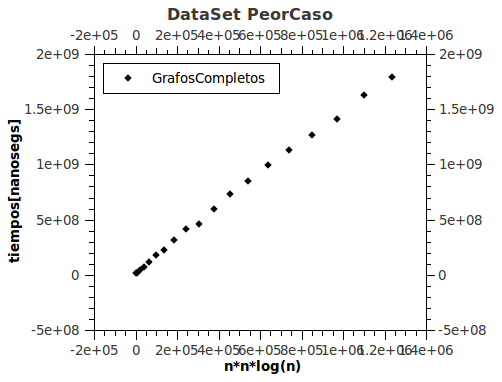
\includegraphics[scale=0.8]{HC/PeorCaso.png}

